\subsection{Beispiel ggT}
\label{sec:Kap-11-2-1}

\begin{figure}[h!]
	\vspace{\baselineskip} %%% für Druck
	\centering
	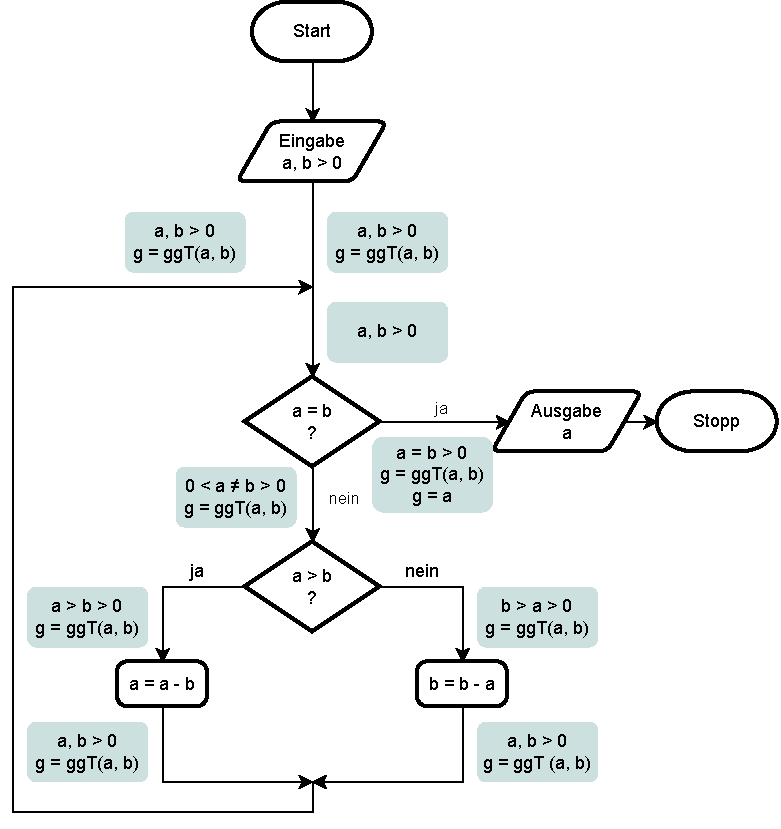
\includegraphics[width=0.9\textwidth]{Bilder/Kapitel-11/Flussdiagramm_Algorithmus_Hoare.pdf}
	\caption{Flussdiagramm mit Zusicherungen}
	\label{fig:flussdiagramm_flgorithmus_hoare}
\end{figure}

Wir betrachten zur Motivation das Flussdiagramm aus Abbildung~\ref{fig:flussdiagramm_flgorithmus_hoare}. Es entspricht dem im vorausgehenden Abschnitt angegebenen Algorithmus~\ref{algo:dritter_reparaturversuch}, also dem letzten Algorithmus zur Berechnung des größten gemeinsamen Teilers zweier Zahlen. Wie kann man verstehen, was dieses Programm macht, ohne seine Abläufe explizit zu betrachten? Wie kann man insbesondere Aussagen zu allen Abläufen machen, obwohl es unendlich viele Abläufe gibt (wir betrachten hier beliebige natürliche Zahlen und beachten nicht, dass kein Rechner unendlich viele unterschiedliche Zahlen darstellen kann)?

Versetzen Sie sich bitte in die Situation, jemand Anderem zu erklären, warum dieses Programm das tut, was es tun soll, also den größten gemeinsamen Teiler der eingegebenen Zahlen $a$ und $b$ bestimmt. Dazu ist es naheliegend, auf gewisse Stellen des Diagramms zu zeigen und anzugeben, was gilt, wenn der Rechner bei der Ausführung „an dieser Stelle ist“. Dafür verwenden wir \emph{Zusicherungen}, 
\marginline{Zusicherungen: Annotationen der Kanten eines Fluss-\\diagramms}
die als \emph{Annotationen} an Kanten geschrieben werden. Diese Beweismethode geht zurück auf Robert Floyd \cite{flo93}.

So wissen wir nach der Eingabe, dass $a > 0$ und $b > 0$ gelten, denn nur dafür ist das Programm gemacht, für andere Eingaben wird nichts gefordert. Deshalb haben wir als erste Annotation an die aus der Eingabe ausgehende Kante diese Eigenschaft von $a$ und $b$ als Zusicherung geschrieben.

Wir verwenden nur für den Zweck der Verifikation eine zusätzliche Variable $g$ (eigentlich eine Konstante), die nicht als Programmvariable zu verstehen ist. Sie enthält das gewünschte Ergebnis laut Spezifikation, also den größten gemeinsamen Teiler von $a$ und $b$. Die später erfolgende Ausgabe sollte dann dem Wert von $g$ entsprechen. Nochmal: $g$ gehört nicht zum Programm und wird auch nicht berechnet, sondern dient hier ausschließlich der Verifikation. Wir können nicht stattdessen $\ggt(a,b)$ verwenden, denn die Werte der Programmvariablen $a$ und $b$ verändern sich während der Programmausführung, und damit potentiell auch $\ggt(a,b)$ (tatsächlich geschieht dies nicht, aber das wird erst zu zeigen sein).

\vspace{1.7mm} %%% für Druck

Anschließend führen zwei Pfeile zusammen, zur ersten Verzweigung $a=b? $ kann man auch über den von links einmündenden Pfeil kommen. Gilt denn auch $a > 0$ und $b > 0$, wenn man von dort kommt? Dies ist zwar der Fall, aber wir können es noch nicht zeigen. Hier kommt nun ein Trick, der mit (den noch einzuführenden) Schleifeninvarianten zusammenhängt: Wir nehmen an, dass auch $a,b > 0$ gilt, wenn wir von links kommen, merken uns aber, dass wir dies später noch begründen müssen.

\vspace{1.7mm} %%% für Druck

Wenn die Bedingung $a = b$ der ersten Verzweigung nicht erfüllt ist, gilt $a < b$ oder $a > b$, sowie weiterhin $a,b >0$. Dies wird an dieser Kante äquivalent und platz\-sparend notiert durch $0<a\neq b >0$. Natürlich gilt weiterhin auch $g = \ggt(a,b)$.

\vspace{1.7mm} %%% für Druck

Die zweite Verzweigung separiert die beiden Fälle $a>b $ und $a<b$, $a=b$ können wir ja hier ausschließen. Links gilt $a > b$, rechts $a < b$. Auf beiden Seiten gilt weiterhin $a,b > 0$.

\vspace{1.7mm} %%% für Druck

Betrachten wir weiter den linken Ast: Da dort $a > b$ gilt, ergibt $a - b$ einen positiven Wert, der $a$ zugewiesen wird. Anschließend gilt also $a > 0$, und natürlich weiterhin $b > 0$. Beim rechten Ast gilt entsprechend ebenfalls nach der Zuweisung $a,b > 0$. Dies gilt also auch nach Zusammenführung der beiden Äste, und die oben „geliehene“ Zusicherung ist damit tatsächlich erfüllt.

\vspace{1.7mm} %%% für Druck

Nun folgt etwas Mathematik. Eine erste Überlegung ist, dass für $a > b$, $\ggt(a,b) = \ggt(a-b,b)$ gilt. Betrachten wir einen gemeinsamen Teiler von $a$ und $b$, also eine Zahl $c$, so dass $a$ und auch $b$ Vielfache von $c$ sind. Dann ist auch $a-b$ Vielfaches von $c$. Umgekehrt gilt: Wenn $a - b$ und $b$ Vielfache von $c$ sind, dann auch $a$ und $b$. Also ist die Menge der gemeinsamen Teiler von $a$ und $b$ identisch mit der Menge der gemeinsamen Teiler von $a - b$ und $b$. Folglich stimmt auch der größte gemeinsame Teiler überein. Entsprechend gilt, für $b > a, \ggt(a,b) = \ggt(a,b-a)$.

\vspace{1.7mm} %%% für Druck

Da $a = a-b$ und $b= b-a$ die einzigen Anweisungen sind, die $a$ oder $b$ verändern, gilt deshalb überall $g = \ggt(a,b)$.

\vspace{1.7mm} %%% für Druck

Eine zweite, einfachere Überlegung ist, dass für $a = b$ gilt: $\ggt(a,b) = \ggt(a,a) = a$. Es gilt $a=b$ beim rechten ausgehenden Pfeil 
der Verzweigung $a=b?$. Daher liefert $a$ den korrekten Wert für $g = \ggt(a,b) = \ggt(a,a) = a$.

\vspace{1.7mm} %%% für Druck

Sind wir mit diesen Überlegungen nun fertig? Tatsächlich lässt sich so zeigen, dass die Ausgabe korrekt ist, wenn sie denn erfolgt. 
\marginline{partielle Korrektheit: jede Ausgabe\\ ist korrekt}
Man nennt diese Eigenschaft \emph{\mbox{partielle} Korrektheit}. Was noch gezeigt werden muss, ist, dass die Ausgabe tatsächlich erreicht wird. Da wir in unserem Programm eine Schleife haben, ist dies ja nicht selbst\-verständlich. Was ist, wenn die Abfrage $a=b?$ stets "`nein"' ergibt und generell, wenn eine Schleife -- für eine bestimmte Eingabe -- nie verlassen wird? Wir nennen eine derartig endlos laufende Schleife \textit{Endlosschleife}.
\marginline{Endlosschleife}

\vspace{1.7mm} %%% für Druck

Wenn wir die partielle Korrektheit bereits gezeigt haben und zusätzlich beweisen können, dass die Ausgabe tatsächlich erreicht wird, dann haben wir die \emph{totale Korrekt\-heit} des Programms bewiesen, und genau das ist unser Ziel. Totale Korrektheit bedeutet, dass die Spezifikation erfüllt ist, wenn wir sie als Zusicherung bei der Ausgabe formuliert haben.

\vspace{1.7mm} %%% für Druck

Wie zeigt man generell, dass eine Schleife irgendwann einmal verlassen wird? Dafür verwendet man meist eine sogenannte \emph{Abstiegsfunktion}. 
\marginline{Abstiegs\-funktion}
Dies ist eine Abbildung der Variablen des Programms auf die natürlichen Zahlen mit der Eigenschaft, dass der Funktionswert bei jedem Schleifendurchlauf abnimmt. Zusätzlich muss gezeigt werden, dass dieser Wert nicht beliebig klein werden kann (so wie es auch keine beliebig kleinen natürlichen Zahlen gibt), also spätestens beim Wert 0 die Schleife verlassen wird. Natürlich hängt diese Abstiegsfunktion stets nur von den Variablenwerten ab, die in der Schleife verändert werden.

\vspace{1.7mm} %%% für Druck

In unserem Beispiel lautet eine geeignete Abstiegsfunktion $f(a,b) = a+b$. Da die Werte von $a$ und $b$ stets positiv bleiben, wird $f(a,b)$ sowohl bei der Anweisung $a = a-b$ als auch bei der Anweisung $b = b-a$ kleiner. Eine der beiden Anweisungen kommt aber bei jedem Schleifendurchlauf vor. Ebenfalls weil $a$ und $b$ stets positiv bleiben, gilt dies für $f(a,b)$. Tatsächlich ist der kleinstmögliche Wert 2, nämlich für $a = b = 1$. Spätestens in diesem Fall wird die Schleife aber verlassen und es wird 1 ausgegeben. Die beiden Eingabewerte waren in diesem Fall teilerfremd. Natürlich kann die Schleife gegebenenfalls auch früher, \dasHeisst bei größeren Werten von $f(a,b)$ verlassen werden.